\documentclass[a4paper,10pt,twocolumn]{ltjarticle}
\usepackage{kaitoushu}

\pgfplotsset{
  myaxis/.style={
    axis lines=middle,
    xlabel={$x$}, ylabel={$y$},
    every axis x label/.style={at={(ticklabel* cs:1)},anchor=west},
    every axis y label/.style={at={(ticklabel* cs:1)},anchor=south},
    tick label style={font=\scriptsize},
    label style={font=\small},
    width=5.5cm, height=5cm,
    grid=none,
    samples=200,
  }
}

\begin{document}

\problemrange{5章：三角関数 — Basic (p.63) 一般角・弧度法・三角関数（問285--299）}



\mondai{285}{次の角を表す動径を図示せよ．}
\kotae{
$360°$で割った余りで位置を判定．

(1) $630°=360°+270°$ → $270°$の位置（$y$軸負方向）

(2) $-310°=50°$（第1象限）

(3) $490°=130°$（第2象限）

(4) $-1120°=-1120+4\times360=320°$（第4象限）

(5) $2000°=2000-5\times360=200°$（第3象限）
}

\mondai{286}{次の角は第何象限の角か．}
\kotae{
(1) $210°$：第3\quad (2) $400°=40°$：第1\quad (3) $-740°=340°$：第4

(4) $820°=100°$：第2\quad (5) $-635°=85°$：第1
}

\mondai{287}{次の三角関数の値を求めよ．}
\kotae{
(1) $\sin210°=-\sin30°=-\dfrac{1}{2}$

(2) $\cos570°=\cos210°=-\dfrac{\sqrt{3}}{2}$

(3) $\tan390°=\tan30°=\dfrac{\sqrt{3}}{3}$

(4) $\sin630°=\sin270°=-1$

(5) $\cos(-225°)=\cos225°=-\dfrac{\sqrt{2}}{2}$

(6) $\tan(-480°)=\tan240°=\sqrt{3}$
}

\mondai{288}{次の角を弧度法で表せ．}
\kotae{
(1) $135°=\dfrac{3\pi}{4}$\quad (2) $36°=\dfrac{\pi}{5}$\quad (3) $-10°=-\dfrac{\pi}{18}$

(4) $240°=\dfrac{4\pi}{3}$\quad (5) $-190°=-\dfrac{19\pi}{18}$
}

\mondai{289}{次の角を60分法で表せ．}
\kotae{
(1) $\dfrac{\pi}{3}=60°$\quad (2) $\dfrac{5\pi}{4}=225°$\quad (3) $-\dfrac{2\pi}{5}=-72°$

(4) $\dfrac{7\pi}{3}=420°$\quad (5) $-\dfrac{\pi}{9}=-20°$
}

\mondai{290}{次の三角関数の値を求めよ．}
\kotae{
(1) $\sin\dfrac{5\pi}{3}=-\sin\dfrac{\pi}{3}=-\dfrac{\sqrt{3}}{2}$

(2) $\cos\dfrac{5\pi}{4}=-\cos\dfrac{\pi}{4}=-\dfrac{\sqrt{2}}{2}$

(3) $\tan\dfrac{\pi}{6}=\dfrac{\sqrt{3}}{3}$
}

\mondai{291}{弧の長さと扇形の面積を求めよ．}
\kotae{
$l=r\theta$，$S=\dfrac{1}{2}r^{2}\theta$

(1) 半径4，中心角$\dfrac{\pi}{6}$：$l=\dfrac{2\pi}{3}$，$S=\dfrac{4\pi}{3}$

(2) 半径3，弧$2\pi$：$\theta=\dfrac{2\pi}{3}$，$S=3\pi$
}

\mondai{292}{次の等式を証明せよ．}
\kotae{
(1) $\tan\theta+\dfrac{1}{\tan\theta}=\dfrac{\sin^{2}\theta+\cos^{2}\theta}{\sin\theta\cos\theta}=\dfrac{1}{\sin\theta\cos\theta}$ \qed

(2) $\dfrac{1}{1-\cos\theta}+\dfrac{1}{1+\cos\theta}=\dfrac{2}{1-\cos^{2}\theta}=\dfrac{2}{\sin^{2}\theta}$ \qed
}

\mondai{293}{象限と1つの三角関数の値から残りを求めよ．}
\kotae{
(1) 第3象限，$\sin\theta=-\dfrac{4}{5}$

$\cos\theta=-\dfrac{3}{5}$，$\tan\theta=\dfrac{4}{3}$

(2) 第4象限，$\cos\theta=\dfrac{1}{3}$

$\sin\theta=-\dfrac{2\sqrt{2}}{3}$，$\tan\theta=-2\sqrt{2}$

(3) 第3象限，$\tan\theta=3$

$\cos\theta=-\dfrac{\sqrt{10}}{10}$，$\sin\theta=-\dfrac{3\sqrt{10}}{10}$
}

\mondai{294}{次の式を簡単にせよ．}
\kotae{
(1) $\cos\theta\sin\!\left(\dfrac{\pi}{2}-\theta\right)+\sin\theta\cos\!\left(\dfrac{\pi}{2}-\theta\right)=\cos^{2}\theta+\sin^{2}\theta=1$

(2) $\sin\!\left(\dfrac{\pi}{2}-\theta\right)-\sin(\pi+\theta)+\cos\!\left(\dfrac{\pi}{2}+\theta\right)+\cos(\pi-\theta)$

$=\cos\theta+\sin\theta-\sin\theta-\cos\theta=0$

(3) $\tan(\pi+\theta)\sin\!\left(\dfrac{\pi}{2}+\theta\right)+\cos(\pi-\theta)\tan(\pi-\theta)$

$=\tan\theta\cos\theta+(-\cos\theta)(-\tan\theta)=\sin\theta+\sin\theta=2\sin\theta$
}

\mondai{295}{次の関数の周期を求め，グラフをかけ．}
\kotae{
(1) $y=\sin\!\left(x-\dfrac{\pi}{2}\right)=-\cos x$\quad 周期$2\pi$

\begin{tikzpicture}
\begin{axis}[myaxis, xmin=-0.5,xmax=7,ymin=-1.5,ymax=1.5,
  xtick={1.5708,3.1416,4.7124,6.2832},
  xticklabels={$\frac{\pi}{2}$,$\pi$,$\frac{3\pi}{2}$,$2\pi$}]
\addplot[thick,blue]{sin(deg(x-1.5708))};
\end{axis}
\end{tikzpicture}

(2) $y=\cos\!\left(x+\dfrac{\pi}{4}\right)$\quad 周期$2\pi$

\begin{tikzpicture}
\begin{axis}[myaxis, xmin=-0.5,xmax=7,ymin=-1.5,ymax=1.5,
  xtick={1.5708,3.1416,4.7124,6.2832},
  xticklabels={$\frac{\pi}{2}$,$\pi$,$\frac{3\pi}{2}$,$2\pi$}]
\addplot[thick,blue]{cos(deg(x+0.7854))};
\end{axis}
\end{tikzpicture}
}

\mondai{296}{次の関数の周期を求め，グラフをかけ．}
\kotae{
(1) $y=2\cos x$\quad 周期$2\pi$，振幅$2$

\begin{tikzpicture}
\begin{axis}[myaxis, xmin=-0.5,xmax=7,ymin=-2.5,ymax=2.5,
  xtick={1.5708,3.1416,4.7124,6.2832},
  xticklabels={$\frac{\pi}{2}$,$\pi$,$\frac{3\pi}{2}$,$2\pi$}]
\addplot[thick,blue]{2*cos(deg(x))};
\end{axis}
\end{tikzpicture}

(2) $y=-\dfrac{1}{2}\sin x$\quad 周期$2\pi$，振幅$\dfrac{1}{2}$

\begin{tikzpicture}
\begin{axis}[myaxis, xmin=-0.5,xmax=7,ymin=-1,ymax=1,
  xtick={1.5708,3.1416,4.7124,6.2832},
  xticklabels={$\frac{\pi}{2}$,$\pi$,$\frac{3\pi}{2}$,$2\pi$}]
\addplot[thick,blue]{-0.5*sin(deg(x))};
\end{axis}
\end{tikzpicture}
}

\mondai{297}{次の関数の周期を求め，グラフをかけ．}
\kotae{
$y=\sin(kx)$ の周期は $\dfrac{2\pi}{|k|}$．

(1) $y=\cos 2x$\quad 周期$\pi$

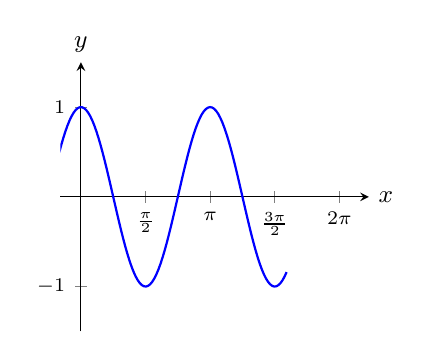
\begin{tikzpicture}
\begin{axis}[myaxis, xmin=-0.5,xmax=7,ymin=-1.5,ymax=1.5,
  xtick={1.5708,3.1416,4.7124,6.2832},
  xticklabels={$\frac{\pi}{2}$,$\pi$,$\frac{3\pi}{2}$,$2\pi$}]
\addplot[thick,blue]{cos(deg(2*x))};
\end{axis}
\end{tikzpicture}

(2) $y=\sin\dfrac{x}{3}$\quad 周期$6\pi$

\begin{tikzpicture}
\begin{axis}[myaxis, xmin=-0.5,xmax=20,ymin=-1.5,ymax=1.5,
  xtick={3.1416,6.2832,9.4248,12.5664,15.708,18.8496},
  xticklabels={$\pi$,$2\pi$,$3\pi$,$4\pi$,$5\pi$,$6\pi$},
  width=6.5cm]
\addplot[thick,blue]{sin(deg(x/3))};
\end{axis}
\end{tikzpicture}
}

\mondai{298}{$0\leqq x<2\pi$ で方程式・不等式を解け．}
\kotae{
(1) $\sin x=\dfrac{\sqrt{2}}{2}$ → $x=\dfrac{\pi}{4},\;\dfrac{3\pi}{4}$

(2) $\cos x=\dfrac{1}{2}$ → $x=\dfrac{\pi}{3},\;\dfrac{5\pi}{3}$

(3) $\sin x\geqq\dfrac{\sqrt{3}}{2}$ → $\dfrac{\pi}{3}\leqq x\leqq\dfrac{2\pi}{3}$

(4) $\cos x<-\dfrac{\sqrt{2}}{2}$ → $\dfrac{3\pi}{4}<x<\dfrac{5\pi}{4}$
}

\mondai{299}{$0\leqq x<2\pi$ で方程式を解け．}
\kotae{
(1) $\tan x=0$ → $x=0,\;\pi$

(2) $\tan x=-1$ → $x=\dfrac{3\pi}{4},\;\dfrac{7\pi}{4}$
}

\end{document}
